\chapter{Phase 2: System Interaktion und Bedienung}

Text Phase 2 kommt hier...

\section{Use Case Diagram}

\section{Sequence Diagram}
Das Interaktionsverhalten für die Szenarien Anruf und Koppeln des Smartwatches mit dem Smartphone, ist fest definiert. Sequenzdiagramme eignen sich zur Kontextabgrenzung sehr gut.\\
In der ~\ref{fig:kopplung} ist der Bluetooth-Kopplungsvorgang als Sequnzdiagramm abgebildet.
Zuerst startet der Smartphone über Bluetooth eine Discovery-Anfrage in der Umgebung.
Das Bluetooth des Smartphones sucht alle verfügbaren Bluetooth-Geräte in der Nähe und übergibt diese dem Smartphone für die Anzeige.
Der Benutzer kann seinen Smartwatch in der Liste auswählen um die Kopplung zu starten.
Danach wird der Benutzer aufgefordert auf seinem Smartphone jetzt die Bluetooth-Kopplungsanforderung mit dem Kopplungs-Code zu bestätigen. Der Kopplungs-Code wird in der Smartwatch angezeigt.
Falls der Benutzer einen falschen Code eingeben hat, wird die Kopplung vom Smartwatch 
abgelehnt.

\begin{figure}[H]
\centering\
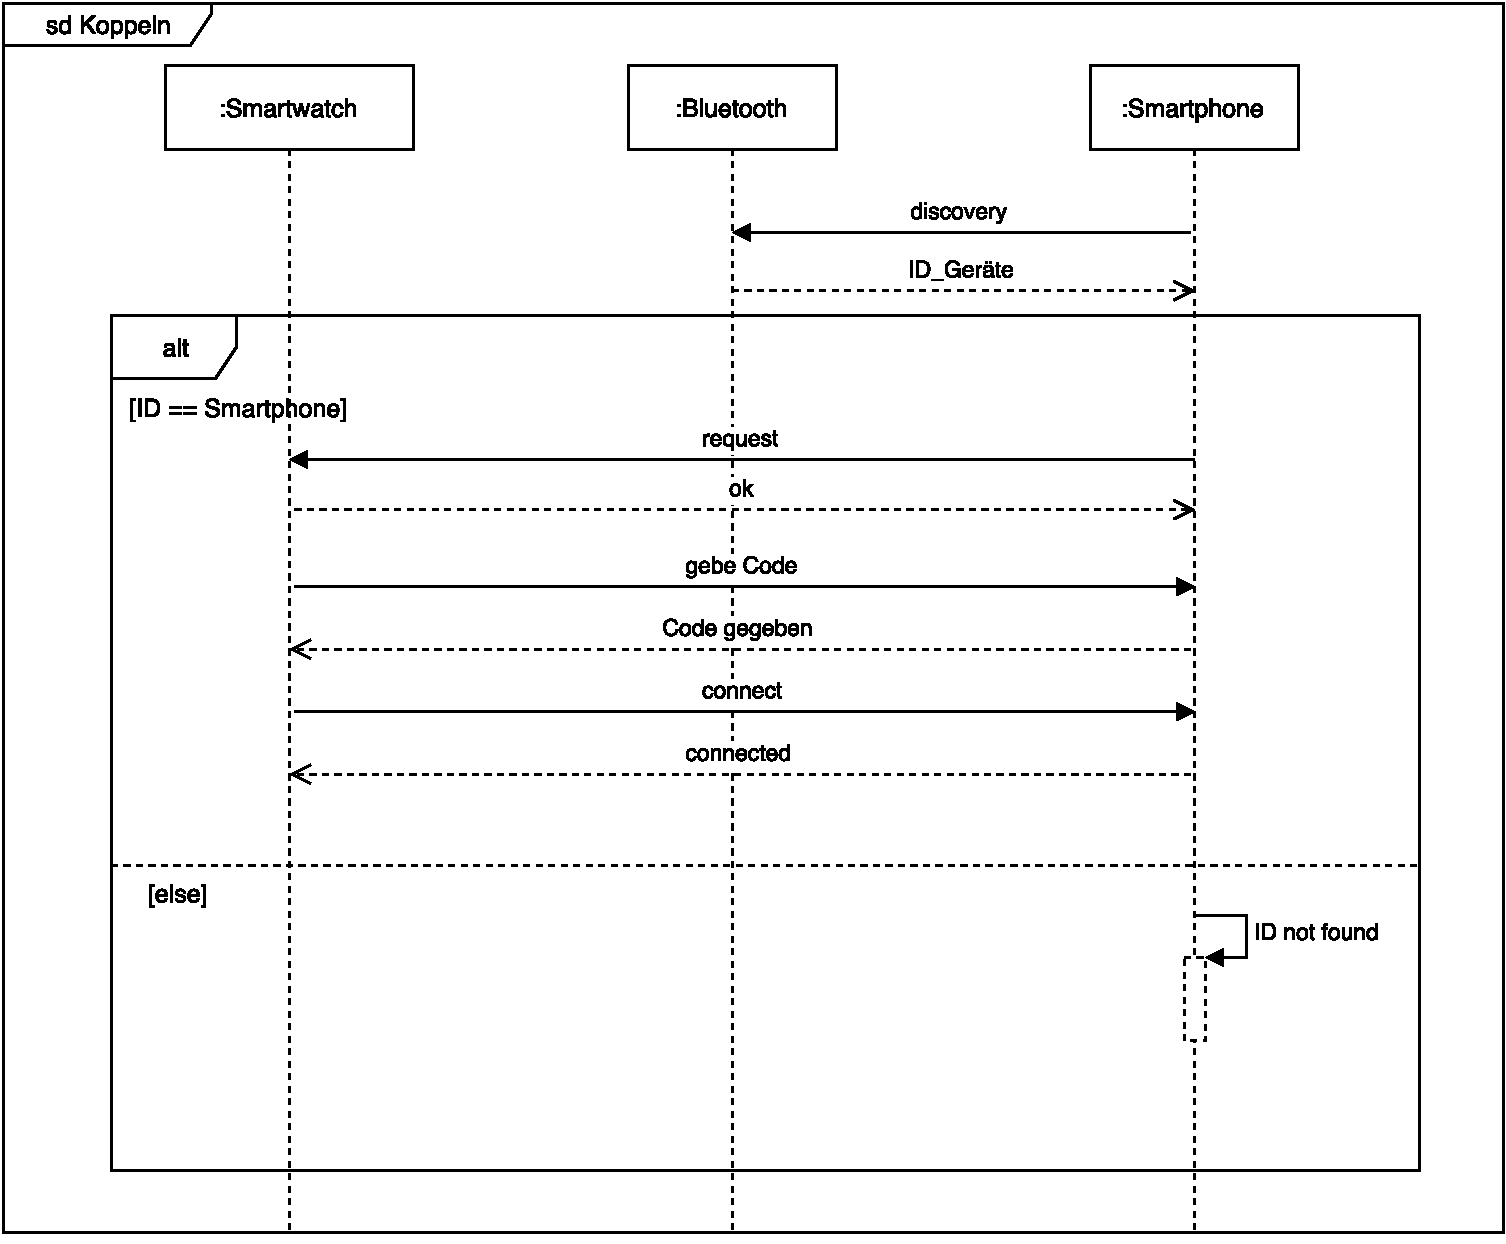
\includegraphics[width=10cm]{img/KoppelnSequenz}
\caption{Kopplung des Smartphones mit Smartwatch}\label{fig:kopplung}
\end{figure}






\section{State Diagram}

\section{Timing Diagram}

